\documentclass[11pt,a4paper]{article}

\usepackage[margin=1in]{geometry}
\usepackage{graphicx}
\usepackage{hyperref}
\usepackage{booktabs}

\title{OpenLeaf Example Article}
\author{Local-first \LaTeX{} editing}
\date{\today}

\begin{document}
% Shared numbers as macros — % Shared numbers as macros — % Shared numbers as macros — \input{metrics} from main.tex
\newcommand{\MetricWordCount}{about 800}
\newcommand{\MetricFigureCount}{1}
\newcommand{\MetricSectionCount}{4}
 from main.tex
\newcommand{\MetricWordCount}{about 800}
\newcommand{\MetricFigureCount}{1}
\newcommand{\MetricSectionCount}{4}
 from main.tex
\newcommand{\MetricWordCount}{about 800}
\newcommand{\MetricFigureCount}{1}
\newcommand{\MetricSectionCount}{4}


\maketitle

\begin{abstract}
A small sample paper that demonstrates the recommended project layout:
\texttt{main.tex}, \texttt{metrics.tex}, \texttt{sections/}, \texttt{figures/},
\texttt{assets/}, \texttt{scripts/}, and \texttt{misc/}.
\end{abstract}

\tableofcontents
\newpage

\section{Introduction}
\label{sec:intro}

This example project shows a typical OpenLeaf layout: a thin \texttt{main.tex},
shared macros in \texttt{metrics.tex}, body text under \texttt{sections/}, and
folders for \texttt{figures/}, \texttt{assets/}, \texttt{scripts/}, and
\texttt{misc/} (notes and other non-compiled material).

OpenLeaf treats the project as a normal filesystem folder---edit any path,
compile with your local TeX engine, and keep sources under version control
(except private projects, which stay gitignored).

\section{Results}
\label{sec:results}

Figure~\ref{fig:flow} is a placeholder image under \texttt{figures/}. Drop binary
assets (images, data dumps) into \texttt{assets/}, put generation or
post-processing helpers in \texttt{scripts/}, and keep scratch notes or drafts
in \texttt{misc/}.

\begin{figure}[ht]
  \centering
  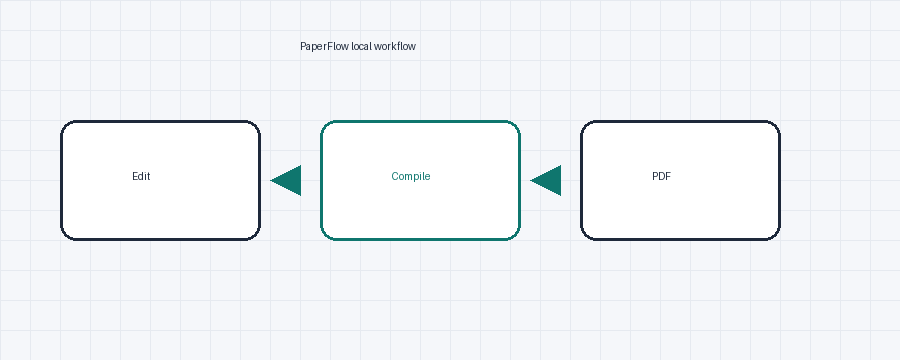
\includegraphics[width=0.72\linewidth]{figures/flow.png}
  \caption{Example figure loaded from the project tree.}
  \label{fig:flow}
\end{figure}

Metrics for this demo: \MetricFigureCount{} figure and \MetricSectionCount{} sections
(\MetricWordCount{} words of fluff).

\section{Discussion}
\label{sec:discussion}

Splitting the manuscript into section files keeps diffs readable and matches how
larger papers are usually organized. Cite prior art with BibTeX as usual~\cite{knuth84,lamport94}.

\section{Methods}
\label{sec:methods}

Compile from the project root (OpenLeaf does this for you). The engine is set in
\texttt{openleaf.json}; override per project or via app config. SyncTeX reverse
search works when the PDF preview is open~\cite{openleaf2026}.


\bibliographystyle{plain}
\bibliography{references}

\end{document}
